\chapter{Transformationen}

\section{Die Hough-Transformation}

Die Hough-Transformation wird verwendet, um Geraden in Bildern zu erkennen. Jede Gerade in einem 
Bild lässt sich eindeutig durch zwei Parameter codieren:
\begin{itemize}
\item Die Richtung der Gerade. Wir suchen dazu nach einem Normalenvektor auf dem Einheitskreis, 
  welcher senkrecht auf die Gerade steht. Jeden Normalenvektor kann man schreiben als
  \[
    v_{\theta} = \begin{pmatrix} \cos(\theta) \\ \sin(\theta) \end{pmatrix},
  \]
  d.h.\ $ \theta $ gibt den Winkel zwischen der $ x $-Achse und dem Vektor $ v_{\theta} $ an. Da es
  zu jeder Gerade offensichtlich zwei Normalenvektoren gibt, beschränken wir uns auf
  $ \theta \in [-\pi / 2, \pi / 2) $, um eine eindeutige Darstellung zu erhalten.
\item Der Abstand $ c \in \R $ der Gerade zum Ursprung. Damit ist die Länge der Strecke gemeint, 
  die durch den Ursprung geht und die Gerade senkrecht schneidet.
\end{itemize}
Die Parametrisierung aller Geraden durch einen Punkt $ x $ des Bildes ist dann gegeben durch
\[
  H(x) = \left\{ 
    (\theta, c) : v_{\theta}^{\top} x = c
  \right\} \subset \left[ -\frac{\pi}{2}, \frac{\pi}{2} \right) \times \R \eqqcolon \mathbb{H}.
\]
Wir betrachten nun eine Menge $ X \subset \R^{2} $ von Punkten (z.B.\ ein Bild) und bilden zu jedem 
der Punkte $ x $ in $ X $ die Menge $ H(x) $. Wir zählen nun, wie oft ein Paar $ (\theta, c) $
insgesamt in den Mengen $ H(x) $ aufgetaucht ist, d.h.\
\[
  n_{X}(\theta, c) \coloneqq \#\{ x \in X : (\theta, c) \in H(x) \}.
\]
Nimmt $ n_{X}(\theta, c) $ einen großen Wert an, dann bedeutet dies, dass wir viele Punkte gefunden
haben, die in einer Linie liegen, sprich eine Gerade bilden. Uns interessiert dabei nicht, welchen
Farb- oder Helligkeitswert die Bildpunkte haben, sondern einfach nur, ob dieser Bildpunkt vorhanden
ist oder nicht. Dazu müssen wir das Bild zuerst binarisieren.

\begin{definition} \leavevmode
\begin{itemize}
\item Ein binarisiertes Bild ist ein Bild, das nur die Werte $ 0 $ oder $ 1 $ annimmt.
  $ 0 $ bedeutet dabei, dass die Farb- oder Grauwertinformation aus dem Originalbild im 
  binarisierten Bild verworfen wird und dieser Bildpunkt im binarisierten Bild \enquote{unsichtbar} 
  sein soll und $ 1 $ bedeutet entsprechend, dass der Bildpunkt aus dem Original auch im 
  binarisierten Bild zu sehen sein soll.
\item Die Hough-Transformation eines endlichen binarisierten Bildes mit Pixeln
  $ X = \{ (x_{j}, y_{j}) \in \R^{2} : j = 1, \ldots, N \} $ ist
  \[
    (H(X))(\theta, c) = n_{X}(\theta, c), \qquad (\theta, c) \in \mathbb{H}.
  \]
\end{itemize}
\end{definition}

Da die meisten Geraden keinen Punkt treffen werden und $ H(X) $ damit fast überall $ 0 $ ist,
zerlegt man $ \mathbb{H} $ normalerweise in kleinere Bereiche $ \mathbb{H}_{jk} $, von denen man
glaubt, dass sie viele Geraden enthalten werden. Dabei ist
$ \mathbb{H}_{jk} \coloneqq \Theta_{j} \times C_{k} $ mit $ j,k = 1, \ldots, M, M' $. $ \Theta_{j} $
ist eine Partition von $ [-\pi / 2, \pi / 2) $ und $ C_{k} $ ist eine Zerlegung eines (hinreichend
großen Teilbereichs) von $ \mathbb{R} $. Damit lässt sich festlegen, in welchen Bereichen des Bildes
man nach welchen Geraden suchen will.

\begin{remark}[Pseudo-Algorithmus zur Diskreten Hough-Transformation] \leavevmode
\begin{enumerate}
\item Gegeben ist ein (beliebiger) Punkt $ p = (x,y) $ des binarisierten Bildes. Wir wollen 
  feststellen, wie viele Geraden durch $ p $ verlaufen.
\item Initialisiere die Matrix $ \mathbf{H} $ mit $ \mathbf{0}_{M \times M'} $. In dieser Matrix
  wird die Häufigkeit codiert, mit der man für ein gegebenes Paar $ (\theta, c) $ den Punkt $ p $
  des Bildes getroffen hat.
\item Für $ j = 1, \ldots, M $:
  \begin{enumerate}
  \item Wähle einen Mittelpunkt $ \theta_{j} $ der Partition $ \Theta_{j} $.
  \item Bestimme einen Index $ k $ mit $ 1 \leq k \leq M' $ so, dass
    \[
      x \cos(\theta_{j}) + y \cos(\theta_{j}) \in C_{k}.
    \]
    D.h., bestimme die Teilbereiche $ C_{k} $ von $ \R $, durch die die Gerade verläuft.
  \item Erhöhe die Anzahl für das entsprechende Paar $ (\theta_{j}, k) $ in der Matrix
  $ \mathbf{H} $ um 1: $ H_{jk} \leftarrow H_{jk} + 1 $.
  \end{enumerate}
\item Ergebnis: $ \mathbf{H} $ ist die diskrete Hough-Transformation.
\end{enumerate}
\end{remark}

Die Matrix $ \mathbf{H} $ kann man nun wiederum als Bild darstellen, indem man die Einträge der
Matrix (die ja Häufigkeiten sind) einfach als Helligkeitswert interpretiert. Die $ x $-Achse des
Bildes gibt den Winkel $ \theta $ der Gerade an, und die $ y $-Achse den Abstand $ c $ der Geraden 
zum Nullpunkt. Ist das Bild an einer Stelle $ (\theta, c) $ hell, so wissen wir, dass die durch
$ (\theta, c) $ codierte Gerade mit hoher Wahrscheinlichkeit eine Gerade in unserem Ursprungsbild
darstellt. Eine andere Möglichkeit, die Ergebnisse der Hough-Transformation zu veranschaulichen,
wäre ein Histogramm zu erstellen, bei dem nach rechts z.B.\ alle Möglichen Paare an Winkel und
Abstand aufgetragen werden und nach oben die Zahl der Punkte, durch die diese Geraden gehen.

\begin{remark}[Vor- und Nachteile der Hough-Transformation] \leavevmode
\begin{itemize}
\item Es werden Kanten erkannt, die in den meisten Fällen eigentlich gar keine Kanten sind, z.B.\ 
  die Ränder des Bildes, oder feine Texturen, wenn der Schwellwert zu niedrig eingestellt ist. 
  Dieser Fehler ist aber leicht zu korrigieren.
\item Die Kanten werden nicht lokalisiert. Wir wissen zwar, durch welche Punkte eine Kante im
  Originalbild verläuft. Wir wissen aber nicht, wo eine Kante tatsächlich beginnt und wo sie endet.
  Dies kann auch ein Vorteil sein, da man so z.B.\ verdeckte Kanten wieder rekonstruieren kann.
\item Bevor die Hough-Transformation auf ein Bild angewendet werden kann, muss dieses binarisiert
  werden. D.h.\ es muss festgelegt werden, welche Pixel des Bildes als potentielle Kanten
  betrachtet werden und welche nicht. Dies geschieht meistens durch Schwellwerte, welche aber durch
  Willkür oder Ausprobieren zustande kommen.
\item Mithilfe der Hough-Transformation lassen sich nicht nur Geraden finden, sondern theoretisch
  alle Kurven, die man irgendwie parametrisieren kann. Z.B.\ kann man Kreise eindeutig durch
  einen Mittelpunkt und Radius darstellen und dies ermöglicht es, mit der Hough-Transformation 
  Kreise im Bild zu finden. Das Problem dabei ist nur, dass mit steigender Zahl an Freiheitsgraden 
  der Aufwand der Transformation \emph{exponentiell} steigt. Je komplexer also die Formen sind,
  nach denen man sucht, desto länger dauert die Transformation. In solchen Fällen hilft es dann nur,
  einen oder mehrere der Freiheitsgrade zu eliminieren, indem man z.B.\ für Kreise einen festen
  Radius oder Mittelpunkt einstellt.
\end{itemize}
Summa summarum: Die Hough-Transformation ist vor allem dann nützlich, wenn man unterbrochene
Kanten im Bild finden will oder das Bild nur durch wenige Kanten dominiert wird.
\end{remark}

\section{Zeit-/Frequenz -- Fenster \& Gabor}

Mit der Fourier-Transformation kann man zwar die in einem Signal enthaltenen Frequenzen analysieren.
Man kann damit aber nicht feststellen, zu welchem Zeitpunkt bzw.\ an welchem Ort des Signals
welche Frequenz auftritt. Ein weiteres Problem besteht in der Fourier-Transformation sehr langer
Signale, was oft die Kapazitäten kleiner Prozessoren in Handys usw.\ übersteigt.

Dies motiviert die Einführung der \emph{Gabor-Transformation}, einer Variante der 
Fourier-Transformation, bei der das Signal in kleineren Stücken durch ein wanderndes 
\enquote{Fenster} betrachtet wird. Denn wenn man die Daten \enquote{fenstert} und nur auf diesem 
Bereich betrachtet, dann sieht man i.W.\ auch nur die Frequenzen, die in diesem Bereich auftreten
und erreicht somit eine bessere Lokalisierung als bei der Fourier-Transformation. Daher wird die 
Gabor-Transformation auch als \enquote{gefensterte Fourier-Transformation} bezeichnet.

\begin{definition}\leavevmode
\begin{itemize}
\item Als \emph{Fensterfunktion} bezeichnen wir eine reelle, gerade und energienormierte Funktion
  $ g \in L_{2}(\R) $, d.h. $ g(x) = g(-x) $ und $ \norm{g}_{2} = 1 $.
\item Wir definieren
  \[
    \phi_{t, \xi}(x) \coloneqq e^{i\xi x} g(x - t), \qquad x \in \R, \quad (t, \xi) \in \R^{2}.
  \]
\item Die Gabor-Transformation zu einer Funktion $ f \in L_{2}(\R) $ ist dann definiert als
  \[
      Gf(t,\xi)
    = \langle f, \phi_{t,\xi} \rangle
    = \int_{\R} f(x) \overline{\phi_{t, \xi}}(x) \dif x
    = \int_{\R} f(x) e^{-i \xi x} g(x - t) \dif x,
      \qquad (t, \xi) \in \R^{2}.
  \]
\end{itemize}
\end{definition}

\begin{remark}
Die Gabor-Transformation liefert also ein Spektogramm $ |Gf| : \R^{2} \rightarrow \R $, das angibt,
wieviel Energie sich zu einem bestimmten Zeitpunkt $ t $ in einer bestimmten Frequenz $ \xi $
konzentriert. Natürlich wird das Spektogramm auch beeinflusst durch die Wahl der Fensterfunktion
$ g $. Wählt man z.B.\ die Rechtecksfunktion, so hat man bedingt durch das Abschneiden wieder mit
Artefakten im Spektogramm zu kämpfen. Wählt man hingegen die Gauß-Funktion, so kann man diesem
Effekt etwas entgegentreten, erhält aber dafür ein Fenster, das \enquote{zu den Rändern} hin immer
milchiger wird. Ein weiterer wichtiger Aspekt ist, dass die Länge des Fensters mit der Periodenlänge
des Signals und der Abtastfrequenz kompatibel sein muss. Sonst kommt es zum sog.\ \enquote{Leck-
Effekt}, bei dem Frequenzen im Spektogramm \enquote{verschmiert} werden.
\end{remark}

\begin{proposition}
Für $ f \in L_{2}(\R) $ gilt:
\begin{description}
\item [Inverse Gabor-Transformation]
  \[
    f(x) = \frac{1}{2\pi} \int_{\R} \int_{\R} Gf(t,\xi) e^{i \xi x} g(x - t) \dif \xi \dif t.
  \]
\item [Parseval-Plancherel]
  \[
    \int_{\R} |f(x)|^{2} \dif x = \frac{1}{2\pi} \int_{\R}\int_{\R} |Gf(t,\xi)|^{2} \dif \xi \dif t.
  \]
  Die Gabor-Transformation auf $ L_{2}(\R) $ im Wesentlichen eine Isometrie.
\end{description}
\end{proposition}

\begin{remark}[Implementierung der Gabor-Transformation]
Unter Verwendung der Identität
\[
    (Gf(\bullet, \xi))^{\wedge}(\omega)
  = \widehat{f}(\omega + \xi)\widehat{g}(\omega)
\]
und damit
\[
    Gf(t, \xi)
  = \left( (Gf(t, \xi))^{\wedge} \right)^{\vee}
  = \left( \widehat{f}(\bullet + \xi) \widehat{g} \right)^{\vee}(t),
\]
kann man die Gabor-Transformation effizient über die FFT implementieren, wenn man $ f $ und $ g $
diskret abtastet.
\end{remark}

Die Gabor-Transformation ist ein Beispiel für die sog.\ \emph{Zeit-Frequenz-Analyse}, bei der man
versucht, die in einem Signal auftretenden Frequenzen zu lokalisieren. Ein weiteres Beispiel ist
Notenschrift, bei der die Form einer Note die zu spielende Dauer und die Lage einer Note die
Tonhöhe, also die Frequenz angibt. Intuitiv müsste man meinen, dass ein kleineres Fenster eine 
bessere Lokalisierung zur Folge hat. Das ist im Grunde genommen auch richtig, aber es gibt gewisse 
\enquote{Grenzen}.

\begin{definition}[Zeit-/Frequenzlokalisierung]
Die \emph{Zeitlokalisierung} einer Funktion $ f \in L_{2}(\R) $ ist als
\[
  \mu = \mu(f) = \frac{1}{\norm{f}_{2}^{2}} \int_{\R} t |f(t)|^{2} \dif t
\]
definiert, die \emph{Frequenzlokalisierung} von $ f $ entsprechend als
\[
    \widehat{\mu} = \widehat{\mu}(f)
  = \frac{1}{\norm{\widehat{f}}_{2}^{2}} \int_{\R} \xi |\widehat{f}(\xi)|^{2} \dif \xi
  = \frac{1}{2\pi \norm{f}_{2}^{2}} \int_{\R} \xi |\widehat{f}(\xi)|^{2} \dif \xi.
\]
Die \emph{Zeitvariation} von $ f $ ist definiert als
\[
  \sigma^{2} = \frac{1}{\norm{f}_{2}^{2}} \int_{\R} (t - \mu)^{2} |f(t)|^{2} \dif t
\]
und entsprechend die \emph{Frequenzvariation} als
\[
    \widehat{\sigma}^{2}
  = \frac{1}{2\pi \norm{f}_{2}^{2}} 
      \int_{\R} (\xi - \widehat{\mu})^{2} |\widehat{f}(\xi)|^{2} \dif \xi.
\]
\end{definition}

\begin{remark}[Heisenberg-Boxen]  \leavevmode
\begin{itemize}
\item Mann kann die Funktionen
  \[
    \frac{|f(t)|^{2}}{\norm{f}_{2}^{2}} \qquad \text{und} \qquad
    \frac{|\widehat{f}(\xi)|^{2}}{\norm{\widehat{f}}_{2}^{2}}
  \]
  als Wahrscheinlichkeitsfunktionen auffassen, denn dann gilt
  \[
    1 = \frac{1}{\norm{f}_{2}^{2}} \int_{\R} |f(t)|^{2} \dif t
      = \frac{1}{\norm{\widehat{f}}_{2}^{2}} \int_{\R} |\widehat{f}(\xi)|^{2} \dif \xi.
  \]
  Die Definition von Erwartungswert $ \mu $ und Varianz $ \sigma^{2} $ ergibt sich dann ganz
  automatisch.
\item Der Wert $ \mu(f) $ ist sozusagen der gewichtete Mittelwert der Energie der Funktion $ f $ im
  Zeitbereich. Analog kann man $ \widehat{\mu}(f) $ als gewichteten Mittelwert der Energie von
  $ \widehat{f} $ im Frequenzbereich betrachten.
\item $ \sigma(f) $ und $ \widehat{\sigma}(f) $ geben an, wie sehr die Funktion von ihrem Mittelwert
  in Zeit und Frequenz abweicht.
\item Eine Funktion hat also ihren Schwerpunkt in Zeit/Frequenz an der Stelle $ (\mu, 
  \widehat{\mu}) $ und die Variationen $ \sigma^{2} $ und $ \widehat{\sigma}^{2} $ geben an, wie 
  gut lokalisiert oder konzentriert die Funktion in Zeit und Frequenz um den Schwerpunkt ist. Den 
  Bereich
  \[
    H(f) \coloneqq 
      [\mu(f) - \sigma(f), \mu(f) + \sigma(f)] \times
      [\widehat{\mu}(f) - \widehat{\sigma}(f), \widehat{\mu}(f) + \widehat{\sigma}(f)]
  \]
  bezeichnet man als \emph{Heisenberg-Box} von $ f $. Eine schematische Darstellung einer solchen
  Box findet sich in Abbildung~\ref{fig:Heisenberg-Box}.
\end{itemize}

\begin{figure}[ht]
\centering
\begin{tikzpicture}
\draw [->] (-0.5,0) -- (7,0) node [right] {$ t $};
\draw [->] (0,-0.5) -- (0,5) node [left] {$ \xi $};
\draw [dashed] (4.5,0) node [below] {$ \mu $} -- (4.5,4.5);
\draw [dashed] (0,3.5) node [left] {$ \widehat{\mu} $} -- (6.5,3.5);
\draw [red] (2.5,2.5) rectangle (6.5,4.5);
\draw [decorate,decoration={brace,mirror,amplitude=5pt},xshift=2pt] 
  (6.5,3.5) -- (6.5,4.5) node [midway,xshift=10pt] { $ \widehat{\sigma} $ };
\draw [decorate,decoration={brace,mirror,amplitude=5pt},yshift=2pt] 
  (6.5,4.5) -- (4.5,4.5) node [midway,yshift=10pt] { $ \sigma $ };
\draw [color=gray, domain=2.5:6.5] plot (\x,{exp(-(\x-4.5)^2)});
\node [color=gray] at (6, 1) {$ \frac{|f(t)|^{2}}{\norm{f}_{2}^{2}} $};
\draw [color=gray, domain=-4.5:-2.5, rotate around={-90:(0,0)}] plot (\x,{exp(-(\x+3.5)^2)-0.35});
\node [color=gray] at (1, 2.5) {$ \frac{|\widehat{f}(\xi)|^{2}}{\norm{\widehat{f}}_{2}^{2}} $};
\end{tikzpicture}
\caption{Schematische Darstellung einer Heisenberg-Box (rot gezeichnet) mit Mittelpunkt
  $ (\mu, \widehat{\mu}) $. Nach rechts aufgetragen ist die Zeit $ t $ und nach oben die Frequenz
  $ \xi $, die zu diesem Zeitpunkt im Signal auftritt. Man sieht, dass die Heisenberg-Box genau die
  Ausdehnung $ [\mu - \sigma, \mu + \sigma] \times
  [\widehat{\mu} - \widehat{\sigma}, \widehat{\mu} + \widehat{\sigma}] $ besitzt, d.h.\
  die Länge $ 2\sigma $ und die Höhe $ 2\widehat{\sigma} $.}
\label{fig:Heisenberg-Box}
\end{figure}
\end{remark}

\begin{proposition}[Heisenberg'sche Unschärferelation]
Für $ f \in L_{2}(\R) $ ist
\[
  \sigma(f)\widehat{\sigma}(f) \geq \frac{1}{2}.
\]
Insbesondere ist sowohl $ \sigma(f) = 0 $ als auch $ \widehat{\sigma}(f) = 0 $ unmöglich.
\end{proposition}

\begin{remark}[Heisenberg'sche Unschärferelation] \leavevmode
\begin{itemize}
\item Die Heisenberg-Boxen können also nicht beliebig klein werden, was nichts anderes heißt, als
  dass es keine beliebig genaue Auflösung sowohl im Frequenz- als auch im Zeitbereich gleichzeitig
  gibt. Jede Heisenberg-Box hat mindestens Fläche $ 2 $. Je genauer
\item Die Heisenberg'sche Unschärferelation liefert außerdem eine Erklärung für unsere 
  Tonwahrnehmung: Ein tiefer Ton besitzt eine geringe Frequenz ($ \rightarrow $ geringe Höhe 
  einer Heisenberg-Box) und daher dauert es vergleichsweise lange ($ \rightarrow $ große Länge der 
  Box), bis der Ton einmal geschwungen ist. Vorher wird der Ton als solcher gar nicht gehört.
  Hohe Tönen hingegen besitzen hohe Frequenzen, dementsprechend kurz ist die Zeit, die der Ton
  braucht, um einmal geschwungen zu sein.
\item Die beste Zeit-/Frequenz-Lokalisierung erreicht man mit den \emph{modulierten Gauß-Funktionen}
  \[
    f(t) = a e^{i \omega t - b(t-u)^{2}} = a e^{i \omega t} e^{-b(t-u)^{2}},
      \qquad u, \omega \in \R, \quad a,b \in \C.
  \]
  In diesem Fall besitzen die Heisenberg-Boxen \emph{exakt} die Fläche $ 2 $.
\end{itemize}
\end{remark}

\TODO{Beispiel zur Gabor-Transformation}

\section{Wavelets}

Da die Gabor-Transformation im Allgemeinen nicht die beste Zeit-/Frequenz-Lokalisierung bieten kann,
wollen wir uns nun mit einer leistungsfähigeren Methode der Zeit-Frequenz-Analyse beschäftigen,
nämlich mit der sog.\ \emph{Kontinuierlichen Wavelet-Transformation}.

\begin{definition}[Wavelets und Zulässigkeit] \leavevmode
\begin{itemize}
\item Eine (möglicherweise komplexwertige) Funktion $ \psi \in L_{2}(\R) $ heißt \emph{Wavelet},
  wenn sie \emph{mittelwertfrei} ist, d.h.\ wenn gilt:
  \[
    \int_{\R} \psi(t) \dif t = 0.
  \]
\item Ein Wavelet $ \psi $ heißt \emph{normalisiert}, wenn $ \norm{\psi}_{2} = 1 $.
\item Ein Wavelet $ \psi $ heißt \emph{zulässig}, wenn
  \[
    C_{\psi} \coloneqq \int_{\R} \frac{|\widehat{\psi}(\xi)|^{2}}{|\xi|} \dif \xi < \infty.
  \]
\end{itemize}
\end{definition}

\begin{remark} \leavevmode
\begin{itemize}
\item Der Name \enquote{Wavelet} (\enquote{Wellchen}) für eine mittelwertfreie Funktion leitet sich
  davon ab, dass diese Funktion Anteile oberhalb und unterhalb der $ x $-Achse haben muss und 
  dadurch eine \enquote{wellenähnliche} Struktur besitzt.
\item Die Zulässigkeitsbedingung sorgt dafür, dass sich $ \widehat{\psi}(\xi) $ am Übergang
  $ \xi \to 0 $ \enquote{brav} verhält, also hinreichend schnell gegen $ 0 $ geht. Das heißt
  insbesondere, dass
  \[
    0 = \widehat{\psi}(0) = \int_{\R} \psi(x) e^{-i \cdot 0 \cdot x} \dif x = \int_{\R} \psi(x) 
    \dif x
  \]
  gelten muss. Daraus folgt sofort, dass jede zulässige Funktion \emph{automatisch} per definitionem
  ein Wavelet ist.
\item Ist das Wavelet $ \psi : \R \rightarrow \R $ reell, so vereinfacht sich die 
  Zulässigkeitsbedingung zu
  \[
    C_{\psi} = \int_{0}^{\infty} \frac{|\widehat{\psi}(\xi)|^{2}}{\xi} \dif \xi < \infty.
  \]
\end{itemize}
\end{remark}

\begin{definition}[Wavelet-Transformation]
Zu einem normalisierten Wavelet $ \psi $ und $ f \in L_{2}(\R) $ ist die Wavelet-Transformation
definiert als
\[
  W_{\psi}f(t, s) \coloneqq
  \int_{\R} f(x) \frac{1}{\sqrt{|s|}} \overline{\psi\left(\frac{x - t}{s}\right)} \dif x, \qquad
    (t,s) \in \R \times \R_{+}.
\]
\end{definition}

\begin{remark} \leavevmode
\begin{itemize}
\item Der Parameter $ t $ verschiebt das Wavelet $ \psi\left(\frac{x - t}{s}\right) $ in der Zeit
  und $ s $ skaliert dieses Wavelet (d.h.\ Streckung oder Stauchung bzgl.\ der $ x $-Achse).
\item Der Term $ 1 / \sqrt{|s|} $ sorgt dafür, dass das Wavelet $ \psi\left(\frac{x - t}{s}\right) $
  normiert ist hinsichtlich der Energienorm.
\end{itemize}
\end{remark}

\begin{example}[Wavelets]
\begin{figure}[ht]
\centering
\begin{minipage}{0.49\textwidth}
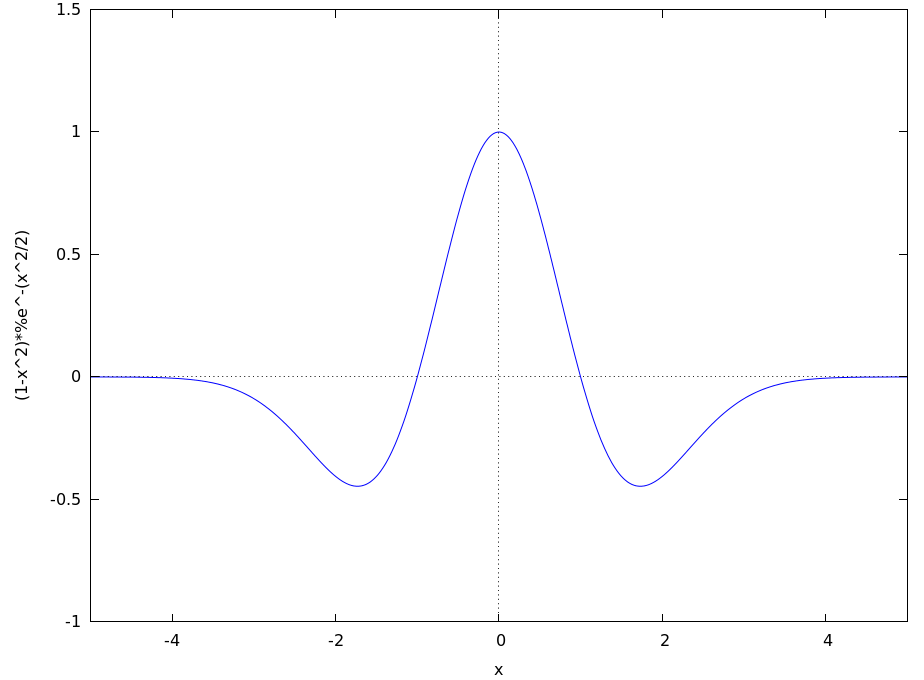
\includegraphics[width=\linewidth]{Bilder/mexican-hat}
\end{minipage}
\hfill
\begin{minipage}{0.49\textwidth}
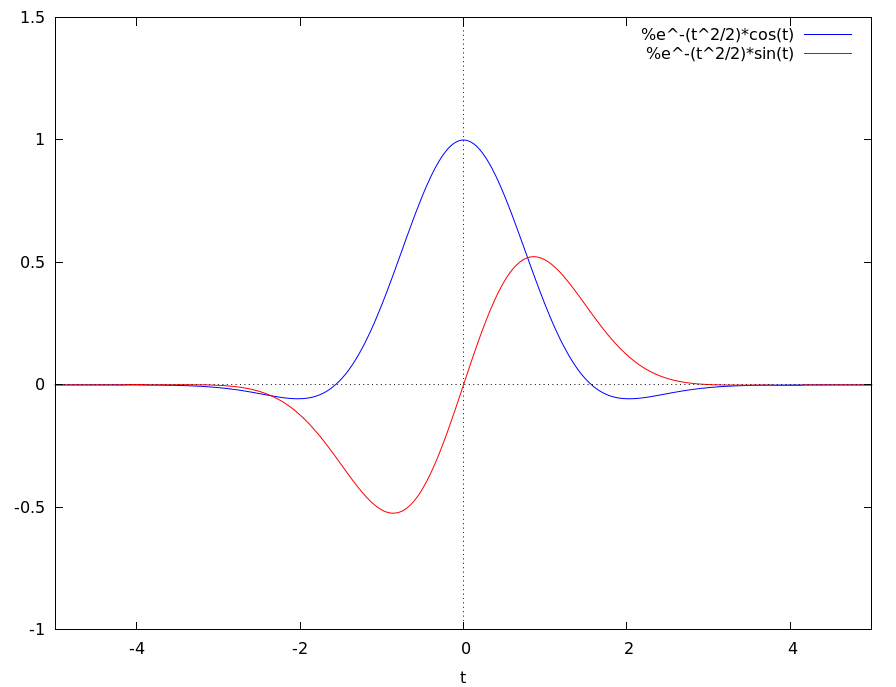
\includegraphics[width=\linewidth]{Bilder/morlet}
\end{minipage}
\caption{Links: Das Mexican-Hat-Wavelet. Rechts: Das Morlet-Wavelet für $ \omega = 1 $ mit
  Real- und Imaginärteil separat gezeichnet (blau bzw.\ rot).}
\label{fig:wavelets}
\end{figure}
\leavevmode
\begin{enumerate}
\item Das \emph{Haar-Wavelet} ist die unstetige Funktion
  \[
    \psi(x) \coloneqq \begin{cases}
      1, & x \in [-1,0), \\
      -1, & x \in (0,1], \\
      0, & \text{sonst}.
    \end{cases}
  \]
\item Das \emph{Mexican-Hat-Wavelet} ist als
  \[
    \psi(t) \coloneqq (1 - t^{2}) e^{-t^{2} / 2} = \dod[2]{}{t} e^{-t^{2} / 2}, \qquad t \in \R
  \]
  definiert. Es besitzt zwar unendlichen Träger, klingt aber exponentiell ab, weshalb es immer noch
  über eine gute Zeitlokalisierung verfügt. Die zugehörige Fourier-Transformierte ist
  \[
    \widehat{\psi}(t) = \sqrt{2\pi} \xi^{2} e^{-\xi^{2} / 2}
  \]
  und damit i.W.\ wieder das Wavelet selbst.
\item Das \emph{Morlet-Wavelet} ist der \enquote{komplexe Bruder} des Mexican-Hat-Wavelets und ist
  definiert als
  \[
    \psi(t) \coloneqq e^{i \omega t} e^{-t^{2} / 2}, \qquad t \in \R, \quad \omega \in \R_{+}.
  \]
  Der Parameter $ \omega $ ist frei wählbar und gibt an, wie oft das Wavelet oszilliert.
  Das Morlet-Wavelet ist nach unserer Definition kein zulässiges Wavelet, da
  \[
    \int_{\R} \psi(t) = \sqrt{2\pi} e^{-\omega^{2} / 2} \neq 0.
  \]
  Wir können aber
  \[
    \widetilde{\psi}(t) \coloneqq \psi(t) - \sqrt{2\pi} e^{-\omega^{2} / 2}
  \]
  setzen, um ein zulässiges Wavelet zu erhalten.
\end{enumerate}
\end{example}

\begin{remark}
Wie wir wissen, bietet uns der modulierte Gauß-Kern die optimale Auflösung hinsichtlich Zeit
\emph{und} Frequenz. Aus diesem Grund verwenden sowohl das Mexican-Hat- als auch das Morlet-Wavelet
die \enquote{Grundfunktion} $ e^{-\bullet^{2} / 2} $.
\end{remark}

\begin{remark}[Skalogramm]
Die Wavelet-Transformation lässt sich in einem sog.\ \emph{Skalogramm} veranschaulichen. Dabei wird
nach rechts die Zeit $ t $ aufgetragen und nach oben die Skalen $ s $. Aber Vorsicht: Die Achse mit
den Skalen ist \enquote{verkehrt herum}, d.h.\ nach oben nehmen die Skalen ab und nach unten nehmen
die Skalen zu. Eine Skala kann man sich vorstellen wie den ungefähren Reziprokwert einer Frequenz.
Farbig codiert ist schließlich der Wert von $ |W_{\psi}f(t,s)| $, d.h.\ mit welcher Intensität eine
Skala $ s $ zum Zeitpunkt $ t $ auftritt.
\end{remark}

Die Zulässigkeit ist eine wichtige Voraussetzung für die Invertierbarkeit der 
Wavelet-Transformation:

\begin{proposition}[Inverse Wavelet-Transformation]
Für ein normalisiertes, zulässiges Wavelet $ \psi $ und eine Funktion $ f \in L_{2}(\R) $ ist
\[
  f(x) = \frac{1}{C_{\psi}} \int_{\R} \int_{\R} W_{\psi} f(t,s)
            \frac{1}{\sqrt{|s|}} \psi\left( \frac{x - t}{s} \right) \dif t \frac{\dif s}{s^{2}}.
\]
\end{proposition}

\begin{remark}[Inverse Wavelet-Transformation] \leavevmode
\begin{itemize}
\item Ist das Wavelet $ \psi $ reell und $ f \in L_{2}(\R) $, dann vereinfacht sich die 
Inversionsformel zu
\[
  f(x) = \frac{1}{C_{\psi}} \int_{0}^{\infty} \int_{\R} W_{\psi} f(t,s)
            \frac{1}{\sqrt{s}} \psi\left( \frac{x - t}{s} \right) \dif t \frac{\dif s}{s^{2}},
\]
wobei natürlich
\[
  C_{\psi} = \int_{0}^{\infty} \frac{|\widehat{\psi}(\xi)|^{2}}{\xi} \dif \xi.
\]
\item Die Umkehrformel gilt nur im $ L_{2} $-Sinn, also eigentlich nicht punktweise.
\item Man kann\footnote{Ich kann es nicht\dots} mathematisch zeigen, dass die 
  Wavelet-Transformation \emph{hochgradig redundant} ist. Dazu stellen wir zunächst fest, dass für 
  die Fourier-Transformation einer \emph{komplexwertigen} Funktion $ f $ gilt
  \[
      \overline{f}^{\wedge}(\xi) 
    = \int_{\R} \overline{f(x)} e^{-i\xi x} \dif x
    = \int_{\R} \overline{f(x)} \overline{e^{i\xi x}} \dif x
    = \overline{\int_{\R} f(x) e^{i\xi x} \dif x}
    = \overline{\widehat{f}(-\xi)}.
  \]
  Bildet man nun die Fourier-Transformierte zur Wavelet-Transformation, dann erhält man
  \[
    (W_{\psi}f(t,s))^{\wedge}(\xi) = \sqrt{s} \widehat{f}(\xi) \widehat{\psi}(s\xi),
  \]
  d.h.\ für zwei Skalen $ s, s' \in \R_{+} $ und eine Frequenz $ \xi $ gilt dann, wenn man obige
  Formel nach $ \widehat{f}(\xi) $ auflöst,
  \[
     \widehat{f}(\xi)
   = \frac{(W_{\psi}f(\bullet,s))^{\wedge}(\xi)}{\sqrt{s}\widehat{\psi}(s\xi)}
   = \frac{(W_{\psi}f(\bullet,s'))^{\wedge}(\xi)}{\sqrt{s'}\widehat{\psi}(s'\xi)}
  \]
  und damit, wenn man nach $ (W_{\psi}f(\bullet,s))^{\wedge}(\xi) $ auflöst,
  \[
      (W_{\psi}f(\bullet,s))^{\wedge}(\xi)
    = \sqrt{\frac{s}{s'}} \frac{\widehat{\psi}(s\xi)}{\widehat{\psi}(s'\xi)}
      (W_{\psi}f(\bullet,s'))^{\wedge}(\xi).
  \]
  Soll heißen: Kennt man die Wavelet-Transformation für \emph{eine} Skala $ s $, dann kann man
  daraus die Wavelet-Transformation für \emph{alle} Skalen $ s' $ herleiten.
\end{itemize}
\end{remark}

Wir kommen nun zum fundamentalen Unterschied zwischen der Gabor-Transformation und der 
Wavelet-Transformation. Dieser hat etwas mit den Heisenberg-Boxen zu tun. Bevor wir dem näher
nachgehen können, müssen wir zunächst noch etwas Vorarbeit leisten.

\begin{definition} \leavevmode
\begin{itemize}
\item Die \emph{Zeit-Frequenz-Atome} zu einem Wavelet $ \psi $ sind definiert als
  \[
    \psi_{t,s} \coloneqq \psi\left(\frac{\bullet - t}{s}\right), \qquad (t,s) \in \R \times \R_{+}.
  \]
\item Ein Wavelet $ \psi $ heißt zentriert, falls
  \[
    \mu(\psi) = 0
  \]
  gilt. Da per definitionem für ein beliebiges $ f \in L_{2}(\R) $ und $ u \in \R $
  \[
      \mu(f(\bullet - u))
    = \int_{\R} t |f(t - u)|^{2} \dif t
    = \int_{\R} (t + u) |f(t)|^{2} \dif t
    = \mu(f) + u
  \]
  gilt, können wir durch geeignete Verschiebung \emph{immer} annehmen, dass $ \psi $ zentriert ist.
\end{itemize}
\end{definition}

Nun zum eigentlichen Satz.

\begin{proposition}
Das Heisenberg-Rechteck $ H(\psi_{t,s}) $ zu einem zentrierten Wavelet $ \psi $ hat den
Mittelpunkt $ (t, \widehat{\mu}(\psi) / s) $ sowie die Seitenlängen $ s \sigma(\psi) $ und
$ \widehat{\sigma}(\psi) / s $.
\begin{figure}[ht]
\centering
\begin{tikzpicture}
\draw [->] (-0.5,0) -- (5,0) node [right] {Zeit};
\draw [<-] (0,-0.5) node [left] {Skala} -- (0,3);
\draw [dashed] (2.5,0) node [below] {$ t $} -- (2.5,2.5);
\draw [dashed] (0,1.5) node [left] {$ \dfrac{\widehat{\mu}}{s} $} -- (4.5,1.5);
\draw [red] (0.5,0.5) rectangle (4.5,2.5);
\draw [decorate,decoration={brace,mirror,amplitude=5pt},xshift=2pt] 
  (4.5,1.5) -- (4.5,2.5) node [midway,xshift=10pt] { $ \dfrac{\widehat{\sigma}}{s} $ };
\draw [decorate,decoration={brace,mirror,amplitude=5pt},yshift=2pt] 
  (4.5,2.5) -- (2.5,2.5) node [midway,yshift=10pt] { $ s\sigma $ };
\end{tikzpicture}
\caption{Ausmaße der Heisenberg-Box bei einem zentrierten Wavelet. Auf der $ x $-Achse ist 
weiterhin die Zeit aufgetragen und auf der $ y $-Achse befinden sich die Skalen. Man beachte
jedoch, dass die $ y $-Achse \enquote{verkehrt herum} ist, d.h.\ niedrige Skalen (welcher hoher
Frequenz entsprechen) sind weiter oben angesiedelt und hohe Skalen (welche niedriger Frequenz
entsprechen) weiter unten.}
\label{fig:Heisenberg-Box-Wavelet}
\end{figure}
\end{proposition}

\begin{remark}
Dieser letzte Satz sagt \emph{alles} über den Unterschied zwischen Gabor-Transformation und
Wavelet-Transformation:
\begin{itemize}
\item Bei der Gabor-Transformation besitzen die Heisenberg-Boxen für die Atome $ \phi_{t,\xi} $ die
  Ausmaße
  \[
    H_{t,\xi} = [t - \sigma(\phi), t + \sigma(\phi)] \times
                [\xi - \widehat{\sigma}(\phi), \xi + \widehat{\sigma}(\phi)].
  \]
  Das heißt, unabhängig von der Skalierung der Fensterfunktion bleibt das 
  \emph{Seitenverhältnis} der Heisenberg-Box \emph{immer unverändert}. Die Gabor-Transformation 
  löst somit \emph{konstant} in Zeit- und Frequenz auf.
\item Die Wavelet-Transformation arbeitet mit \emph{adaptiver} (oder relativer)
  Zeit-Frequenz-Auflösung, d.h.\ das Seitenverhältnis der Heisenberg-Box ändert sich dynamisch.
  Besitzt ein Signal sowohl niedrige als auch hohe Frequenzen, dann möchte man\dots
  \begin{itemize}
  \item in Bereichen hoher Frequenz (also bei kleinen Werten des Skalenparameters $ s $) eine gute 
    Auflösung in Ort/Zeit haben. Denn in hohen Frequenzen stecken die Details eines Signals, und
    von denen möchte man genau wissen, wo sie sich befinden. Wegen der Heisenberg'schen
    Unschärferelation ist dafür die Auflösung im Frequenzbereich geringer, sodass man nicht genau 
    bestimmen kann, wie die Details aussehen.
  \item in Bereichen niedriger Frequenz (also bei großen Werten von $ s $) eine gute Auflösung
    im Frequenzbereich haben. Denn in den niedrigen Frequenzen stecken die einflussreichen groben 
    Informationen eines Signals. Deshalb möchte man hier genau wissen, welche Werte diese annehmen.
    Eine gute Auflösung in Ort/Zeit hingegen ist nicht so wichtig, weil die niedrigen Frequenzen
    nur langsam schwingen und sich daher lokal weniger ändert.
  \end{itemize}
  Man wünscht sich also bei niedrigen Frequenzen eine gute Frequenzauflösung unter Inkaufnahme 
  einer schlechten Zeitauflösung und bei hohen Frequenzen eine gute Zeitauflösung bei schlechterer 
  Frequenzauflösung. Genau das leistet die Wavelet-Transformation. Dieser Sachverhalt ist auch in
  Abbildung~\ref{fig:Heisenberg-Box-Wavelet-Anpassung} veranschaulicht. Die Gabor-Transformation 
  leistet beides nicht.
  \begin{figure}[ht]
  \centering
  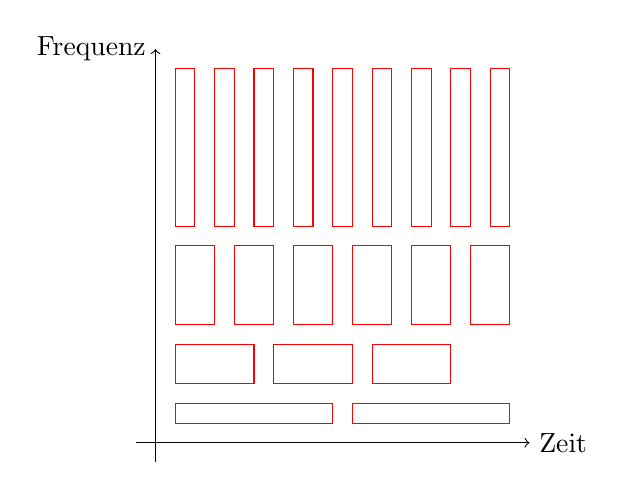
\begin{tikzpicture}[scale=0.5]
  \draw [->] (-0.5,0) -- (9.5,0) node [right] {Zeit};
  \draw [->] (0,-0.5) -- (0,10) node [left] {Frequenz};
  
  \draw [red] (0.5,0.5) rectangle (4.5,1);
  \draw [red] (5,0.5) rectangle (9,1);
  
  \draw [red] (0.5,1.5) rectangle (2.5,2.5);
  \draw [red] (3,1.5) rectangle (5,2.5);
  \draw [red] (5.5,1.5) rectangle (7.5,2.5);
  
  \draw [red] (0.5,3) rectangle (1.5,5);
  \draw [red] (2,3) rectangle (3,5);
  \draw [red] (3.5,3) rectangle (4.5,5);
  \draw [red] (5,3) rectangle (6,5);
  \draw [red] (6.5,3) rectangle (7.5,5);
  \draw [red] (8,3) rectangle (9,5);
  
  \draw [red] (0.5,5.5) rectangle (1,9.5);
  \draw [red] (1.5,5.5) rectangle (2,9.5);
  \draw [red] (2.5,5.5) rectangle (3,9.5);
  \draw [red] (3.5,5.5) rectangle (4,9.5);
  \draw [red] (4.5,5.5) rectangle (5,9.5);
  \draw [red] (5.5,5.5) rectangle (6,9.5);
  \draw [red] (6.5,5.5) rectangle (7,9.5);
  \draw [red] (7.5,5.5) rectangle (8,9.5);
  \draw [red] (8.5,5.5) rectangle (9,9.5);
  \end{tikzpicture}
  \caption{Die schematische Darstellung der Heisenberg-Boxen zu einem Wavelet. Nach oben (also
  zu höheren Frequenzen und damit kleineren Skalen) werden die Rechtecke schmäler und höher. Dadurch
  verbessert sich die Auflösung im Zeitbereich auf Kosten der Auflösung im Frequenzbereich. Nach 
  unten
  hin (kleinere Frequenzen und damit größere Skalen) werden die Rechtecke breiter und niedriger. Die
  Auflösung im Frequenzbereich verbessert sich auf Kosten der Auflösung im Zeitbereich.}
  \label{fig:Heisenberg-Box-Wavelet-Anpassung}
  \end{figure}
\item Die Heisenberg-Boxen zu einem Wavelet haben alle dieselbe Fläche, nämlich
  \[
    2s\sigma \cdot 2\frac{\widehat{\sigma}}{s} = 4 \sigma \widehat{\sigma}.
  \]
\end{itemize}
\end{remark}

\subsection{Die Implementierung der Wavelet-Transformation}
That's too nerdy for me\dots

\subsection{Inverse Transformation \& Pferdefüße}
That's too nerdy for me\dots

\subsection{Beispiele -- Musik und Kanten}
That's too nerdy for me\dots

Und noch eine Definition, die ich hier einfach so einstreue, weil wir mal eine Übungsaufgabe dazu
gemacht haben, auch wenn dies nicht unmittelbar hier her passt:

\begin{definition}
Ein Wavelet $ \psi $ besitzt $ n $ verschwindende Momente, wenn
\[
  \int_{\R} t^{k} \psi(t) \dif t = 0, \qquad k = 0, \ldots, n-1.
\]
\end{definition}

\begin{remark}\leavevmode
\begin{itemize}
\item Das Wavelet $ \psi' $ hat dann übrigens $ n + 1 $ verschwindende Momente.
\item Das Haar-Wavelet hat genau ein verschwindendes Moment (siehe Übung).
\item Wozu soll das überhaupt gut sein? Ich hab keine Ahnung, aber soweit ich das beurteilen kann
  scheint das irgendwas mit der Analyse eines Skalogramms zu tun haben (?)
\end{itemize}
\end{remark}

\section{Filterbänke}

Filterbänke verwenden die Idee des sog.\ \emph{Subband Coding}. Dabei wird das Signal in mehrere
Teilsignale (\emph{Subbänder}) aufgespalten, welche dann separat weiterverarbeitet werden, z.B.\ 
mit der Wavelet-Transformation. Natürlich sollte aus den Subbändern auch wieder das ursprüngliche
Signal rekonstruiert werden können. Dazu brauchen wir erst wieder etwas mathematische Theorie.

\begin{definition}[z-Transformation]
Die \emph{z-Transformation} eines diskreten Signals $ c \in l_{1}(\Z) $ ist die formale 
Laurent-Reihe
\[
  c^{*}(z) \coloneqq \sum_{k \in \Z} c(k) z^{-k}, 
    \qquad z \in \C_{\times} \coloneqq \C \setminus \{ 0 \}.
\]
\end{definition}

\begin{remark}[z-Transformation]
Die z-Transformation kann als Verallgemeinerung der Diskreten Fourier-Transformation angesehen 
werden. Schließlich gilt ja für beliebiges $ \theta \in \T $
\[
    c^{*}(e^{i\theta})
  = \sum_{k \in \Z} c(k) \left( e^{i\theta} \right)^{-k}
  = \sum_{k \in \Z} c(k) e^{-i\theta k}
  = \widehat{c}(\theta).
\]
Beispielsweise gilt auch für $ c, d \in l_{1}(\Z) $
\[
  (c * d)^{*}(z) = c^{*}(z) d^{*}(z).
\]
\end{remark}

Nun wäre die naheliegendste Idee, für die Subband-Zerlegung das Signal mittels verschiedener 
nicht überlappender Bandpassfilter (charakteristische Funktionen) aufzuspalten. Dies mit 
LTI-Filtern zu realisieren ist aber weder alles andere als einfach, noch effizient. Daher wollen 
wir uns nun eine einfachere und praktikablere Zerlegung ansehen.

\begin{definition}
Sei $ n \geq 2 $. Der Operator $ \downarrow_{n} $, der eine Folge $ c \in l(\Z) $ abbildet auf
\[
  \downarrow_{n} c = c(n \cdot \bullet),
\]
heißt \emph{Downsampling-Operator} der Ordnung $ n $. Der Operator $ \uparrow_{n} $ mit
\[
  \uparrow_{n} c(j) = \begin{cases}
    c(j / n), & j \in n\Z \\
    0, & j \in Z \setminus n\Z,
  \end{cases}
\]
heißt \emph{Upsampling-Operator} der Ordnung $ n $.
\end{definition}

\begin{remark}\leavevmode
\begin{itemize}
\item Der Downsampling-Operator der Ordnung $ n $ behält also nur jeden $ n $-ten Eintrag eines 
  Signals. Der Upsampling-Operator \enquote{bläst} das Signal künstlich auf, indem er zwischen die 
  bereits vorhandenen Einträge einfach $ n - 1 $ weitere $ 0 $-Einträge setzt. Beispiel: Aus der
  Folge
  \[
    c \coloneqq \begin{bmatrix} 1 & 2 & 3 & 4 & 5 \end{bmatrix}
  \]
  gewinnt man mittels Downsampling der Ordnung $ 2 $
  \[
    \downarrow_{2} c = \begin{bmatrix} 1 & 3 & 5 \end{bmatrix}
  \]
  und mittels Upsampling der Ordnung $ 2 $
  \[
    \uparrow_{2} c = \begin{bmatrix} 1 & 0 & 2 & 0 & 3 & 0 & 4 & 0 & 5 \end{bmatrix}.
  \]
\item In der Operatorschreibweise liest man von rechts nach links, d.h. bei
  $ \downarrow_{n} \uparrow_{n} c $ wird zuerst $ \uparrow_{n} $ und dann $ \downarrow_{n} $
  ausgeführt.
\item Offensichtlich gilt:
  \[
    \downarrow_{n} \uparrow_{n} = I \neq{} \uparrow_{n} \downarrow_{n}.
  \]
  Denn auf der linken Seite wird zuerst mit Nullen aufgefüllt, welche dann wieder entfernt werden.
  Auf der rechten Seite werden allerdings alle $ n $-ten Einträge entfernt, welche dann durch Nullen
  ersetzt werden.
\end{itemize}
\end{remark}

Mithilfe des Downsampling-Operators der Ordnung $ n $ kann man nun ein Signal $ c $ in die $ n $ 
Subbänder
\[
  c_{j} \coloneqq{} \downarrow_{n} \tau_{j} c, \qquad j \in \Z_{n}
\]
zerlegen, welche man mit der Formel
\[
  c = \sum_{j \in \Z_{n}} \tau_{j} \uparrow_{n} c_{j}
\]
wieder zu $ c $ kombinieren kann. Beispiel: Angenommen, wie haben ein $ 9 $-periodisches Signal
$ c $ mit den Einträgen
\[
  c = \begin{bmatrix} 1 & 2 & 3 & 4 & 5 & 6 & 7 & 8 & 9 \end{bmatrix},
\]
dann erhalten wir durch Translation um $ 0,1,2 $ und jeweils Downsampling der Ordnung $ 3 $ die 
drei Subbänder
\[
c_{0} \coloneqq \begin{bmatrix} 1 & 4 & 7 \end{bmatrix}, \quad
c_{1} \coloneqq \begin{bmatrix} 2 & 5 & 8 \end{bmatrix}, \quad
c_{2} \coloneqq \begin{bmatrix} 3 & 6 & 9 \end{bmatrix},
\]
sodass $ c_{j} = c(n \cdot \bullet + j) $ für ein $ j \in \Z_{3} $.
Upsampling der Ordnung $ 3 $ und Translation um $ 0,1,2 $ liefern mit anschließender Addition wieder
das Ausgangssignal:
\[
  \begin{array}{*{9}{c}}
  1 & 0 & 0 & 4 & 0 & 0 & 7 & 0 & 0 \\
  0 & 2 & 0 & 0 & 5 & 0 & 0 & 8 & 0 \\
  0 & 0 & 3 & 0 & 0 & 6 & 0 & 0 & 9 \\ \hline
  1 & 2 & 3 & 4 & 5 & 6 & 7 & 8 & 9
  \end{array}
\]

Das Subband-Coding verallgemeinert dieses Prinzip. Statt des Translationsoperators verwenden wir
jetzt einfach $ n $ allgemeine Filter $ F_{j} $, $ j \in \Z_{n} $, und wenden auf jedes der 
Resultate den Downsampling-Operator an:
\[
  c_{j} ={} \downarrow_{n} F_{j} c, \qquad j \in \Z_{n}.
\]
Schematisch:
\[
  \begin{array}{*{9}{c}}
  & & & \nearrow & \boxed{F_{0}} & \rightarrow & \boxed{\downarrow_{n}} & \rightarrow & c_{0} \\
  c & \rightarrow & \odot & & \vdots & & \vdots & & \vdots \\
  & & & \searrow & \boxed{F_{n-1}} & \rightarrow & \boxed{\downarrow_{n}} & \rightarrow & c_{n-1}
  \end{array}
\]
Diese Zerlegung bezeichnet man als \emph{Analyse-Filterbank} $ F = (F_{j} : j \in \Z_{n}) $. Wir 
haben dabei die Anzahl der Subbänder gleich der Ordnung des Downsampling-Operators gewählt. Solche
Filterbänke bezeichnet man als \emph{kritisch abgetastet}. Ist die Anzahl der Subbänder kleiner als
die Ordnung des Downsamplings, dann spricht man von \emph{Unterabtastung}. Eine solche Filterbank
wurde bereits oben anhand des Translationsoperators gezeigt. Ist die Zahl der Subbänder größer als
die Ordnung des Downsamplings, so spricht man von \emph{Überabtastung}.

Wir werden nun sehen, dass sich jede Analyse-Filterbank als Matrix beschrieben lässt. Dabei kommt
endlich die z-Transformation ins Spiel. Dabei nehmen wir an, dass jeder Filter $ F_{j} $ ein
LTI-Filter mit Impulsantwort $ f_{j} $ ist, dass also $ F_{j}c = f_{j} * c $ gilt.

\begin{definition}[Modulationsmatrix]
Die \emph{Modulationsmatrix} $ M(z) $ zu der Filterbank
\[
  F = (F_{j} : j \in \Z_{n})
\]
ist definiert als
\begin{align*}
   M(z)
  &\coloneqq \frac{1}{n} \left( f_{j}^{*} \left( e^{2\pi ik/n} \right) : j,k \in \Z_{n} \right) \\
  &= \frac{1}{n} \begin{pmatrix}
    f_{0}^{*}(z) & f_{0}^{*}(e^{2\pi i/n}) & \cdots & f_{0}^{*}(e^{2\pi i(n-1)/n} \\
    \vdots & \vdots & \ddots & \vdots \\
    f_{n-1}^{*}(z) & f_{n-1}^{*}(e^{2\pi i/n}) & \cdots & f_{n-1}^{*}(e^{2\pi i(n-1)/n})
  \end{pmatrix}.
\end{align*}
\end{definition}

\begin{remark}[Modulationsmatrix] \leavevmode
\begin{itemize}
\item Für $ n = 2 $ hat die Modulationsmatrix die Gestalt
  \[
    M(z) = \frac{1}{2}
    \begin{pmatrix}
      f_{0}^{*}(z) & f_{0}^{*}(-z) \\
      f_{1}^{*}(z) & f_{1}^{*}(-z)
    \end{pmatrix}.
  \]
\item Die Vorfaktoren $ e^{2\pi ik/n} $ vor der Variablen $ z $ sind $ n $-te Einheitswurzeln und
  spielen daher die Rolle verallgemeinerter Vorzeichen.
\item Die Bedeutung der Modulationsmatrix liegt darin, dass sie die Filterbank beschreibt.
\end{itemize}
\end{remark}

\begin{example}[Modulationsmatrix für die Translationsfilter]
Wir berechnen die Modulationsmatrix für die Translationsfilter $ F_{j} = \tau_{j} $,
$ j \in \Z_{n} $. Dazu bestimmen wir als Erstes die Impulsantwort $ f_{j} $ für $ F_{j} $. Es gilt
\[
  f_{j} = F_{j}\delta = \tau_{j}\delta = \delta(\bullet + j).
\]
Die z-Transformation der Impulsantwort ist damit für ein $ z \in \C_{\times} $ gegeben durch
\[
    f_{j}^{*}(z)
  = \sum_{k \in \Z} f_{j}(k) z^{-k}
  = \sum_{k \in \Z} \delta(k + j) z^{-k}
  = \begin{cases}
      0, & k \neq -j, \\
      z^{j}, & k = -j
    \end{cases}
  = z^{j}.
\]
Die Modulationsmatrix $ M(z) $ zur Filterbank $ F = (F_{j} : j \in \Z_{n}) $ ist schließlich
\begin{align*}
   M(z)
&= \frac{1}{n} \left( f_{j}^{*}(e^{2\pi ik/n}) : j,k \in \Z_{n} \right) 
 = \frac{1}{n} \begin{pmatrix}
     1 & 1 & \cdots & 1 \\
     \vdots & \vdots & \ddots & \vdots \\
     z^{n-1} & \left( e^{2\pi i/n}z \right)^{n-1} & \cdots & \left( e^{2\pi i(n-1)/n}z \right)^{n-1}
   \end{pmatrix}.
\end{align*}
\end{example}

\begin{definition}[Polyphasen-Vektor]
Der Vektor
\[
  \left( c^{*}(e^{2\pi ik/n}z) : k \in \Z_{n} \right)
\]
zu einem Signal $ c $ heißt \emph{Polyphasen-Vektor} zu $ c $.
\end{definition}

\begin{proposition}
Für die Analyse-Filterbank gilt
\[
    \left( c^{*}_{k}(z^{n}) : k \in \Z_{n} \right)
  = M(z) \left( c^{*}(e^{2\pi ik/n}z) : k \in \Z_{n} \right).
\]
Das heißt
\[
    \begin{pmatrix}
      c_{0}^{*}(z^{n}) \\
      c_{1}^{*}(z^{n}) \\
      \vdots \\
      c_{n-1}^{*}(z^{n})
    \end{pmatrix}
  = M(z) \begin{pmatrix}
      c^{*}(z) \\
      c^{*}(e^{2\pi i/n}z) \\
      \vdots \\
      c^{*}(e^{2\pi i(n-1)/n}z)
    \end{pmatrix}
\]
\end{proposition}

\begin{remark} \leavevmode
\begin{itemize}
\item Das Ergebnis einer Filterbank lässt sich also berechnen, indem man die Modulationsmatrix der
  Filterbank mit dem Polyphasen-Vektor des Signals multipliziert.
\item Für den Fall $ n = 2 $ gilt
  \[
    \begin{pmatrix}
      c_{0}^{*}(z^{2}) \\
      c_{1}^{*}(z^{2})
    \end{pmatrix}
  = \frac{1}{2}
    \begin{pmatrix}
      f_{0}^{*}(z) & f_{0}^{*}(-z) \\
      f_{1}^{*}(z) & f_{1}^{*}(-z)
    \end{pmatrix}
    \begin{pmatrix}
      c^{*}(z) \\
      c^{*}(-z)
    \end{pmatrix}.
  \]
\end{itemize}
\end{remark}

Nun wollen wir den Analyseprozess umkehren und die Subbänder $ c_{j} $, $ j \in \Z_{n} $ wieder zu
einem Signal $ c $ zusammensetzen. Dazu gehen wir genau den umgekehrten Weg und führen erst ein
Upsampling jedes Subbandes durch, filtern das Ergebnis mit den entsprechenden Filtern $ G_{j} $,
$ j \in \Z_{n} $ und summieren die Resultate schließlich auf. Also:
\[
  c' = \sum_{k \in \Z_{n}} G_{j} \uparrow_{n} c_{j}.
\]
Dies führt uns zur \emph{Synthese-Filterbank}
\[
  \begin{array}{*{9}{c}}
    c_{0} & \rightarrow & \boxed{\uparrow_{n}} & \rightarrow & \boxed{G_{0}} & \searrow & & \\
    \vdots & & \vdots & & \vdots & & \oplus & \rightarrow & c' \\
    c_{n-1} & \rightarrow & \boxed{\uparrow_{n}} & \rightarrow & \boxed{G_{n-1}} & \nearrow & &
  \end{array}
\]
mit der Modulationsmatrix
\[
  \widetilde{M}(z) = \begin{pmatrix}
    g_{0}^{*}(z) & \cdots & g_{n-1}^{*}(z) \\
    \vdots & \ddots & \vdots \\
    g_{0}^{*}(e^{2\pi i(n-1)/n}) & \cdots & g_{n-1}^{*}(e^{2\pi i(n-1)/n})
  \end{pmatrix}.
\]
Das heißt
\[
    \left( c^{*}(e^{2\pi ik/n}z) : k \in \Z_{n} \right)
  = \widetilde{M}(z) \left( c^{*}_{k}(z^{n}) : k \in \Z_{n} \right).
\]
Auf der linken Seite erhalten wir also wieder genau den Polyphasen-Vektor, den wir anfangs mit der 
Modulationsmatrix der Analyse-Filterbank multipliziert haben.

Was wir aber letztendlich betrachten wollen sind nicht die Analyse- oder Synthese-Filterbank für 
sich alleine genommen, sondern das Gesamtsystem, die \emph{Filterbank}, die wir erhalten, wenn wir
Analyse- und Synthese-Filterbank zusammenstöpseln:
\[
  \begin{array}{*{17}{c}}
    & & & \nearrow & \boxed{F_{0}} & \rightarrow & \boxed{\downarrow_{n}} & \rightarrow & c_{0} 
        & \rightarrow & \boxed{\uparrow_{n}} & \rightarrow & \boxed{G_{0}} & \searrow & & \\
    c & \rightarrow & \odot & & \vdots & & \vdots & & \vdots 
        & & \vdots & & \vdots & & \oplus & \rightarrow & c' \\
    & & & \searrow & \boxed{F_{n-1}} & \rightarrow & \boxed{\downarrow_{n}} & \rightarrow & c_{n-1}
        & \rightarrow & \boxed{\uparrow_{n}} & \rightarrow & \boxed{G_{n-1}} & \nearrow & &
  \end{array}
\]
Dabei sollte hinten wieder dasselbe herauskommen, was man vorne hineingesteckt hat.

\begin{definition}[Perfekte Rekonstruktion]
Die Filterbank $ (F,G) $ liefert \emph{perfekte Rekonstruktion}, wenn $ c' = c $ für alle
Eingabedaten $ c $ gilt.
\end{definition}

\begin{remark}[Perfekte Rekonstruktion]\leavevmode
\begin{itemize}
\item Unter Verwendung der Modulationsmatrizen für Analyse- und Synthese-Filterbank kann man
  perfekte Rekonstruktion auch schreiben als:
  \[
      \left( c^{*}(e^{2\pi ik/n}z) : k \in \Z_{n} \right)
    = \widetilde{M}(z) M(z)
      \left( c^{*}(e^{2\pi ik/n}z) : k \in \Z_{n} \right).
  \]
  Da links und rechts zwei identische Polyphasen-Vektoren stehen, folgt sofort
  \[
    \widetilde{M}(z) M(z) = I, \qquad \widetilde{M}(z) = M^{-1}(z).
  \]
  Damit ist die \emph{komplette} Filterbank bereits durch die Modulationsmatrix der
  Analyse-Filterbank festgelegt.
\item Manchmal erlaubt man der Filterbank auch, dass die Originaldaten zeitverzögert rekonstruiert
  werden, d.h.\ $ c' = \tau_{k} c $ für ein $ k \in \Z $. Das ist zwar streng genommen keine
  perfekte Rekonstruktion mehr, aber aus $ \tau_{k} c $ lässt sich $ c $ ja leicht wieder gewinnen.
\item Es ist
  \[
    \widetilde{M}(z) M(z) =
    \left( 
      \sum_{l \in \Z} g_{l}^{*}(e^{2\pi ij/n}z) f_{l}^{*}(e^{2\pi ik/n}z) : j,k \in \Z_{n}
    \right).
  \]
\end{itemize}
\end{remark}

Wir wissen jetzt, dass perfekte Rekonstruktion aus $ \widetilde{M}(z) M(z) = I $ folgt. Interessant
ist, dass auch die Umkehrung gilt.

\begin{proposition}[Perfekte Rekonstruktion]
Eine Filterbank $ (F,G) $ besitzt die Fähigkeit zur perfekten Rekonstruktion genau dann, wenn
\[
  \widetilde{M}(z) M(z) = I, \qquad z \in \C.
\]
\end{proposition}